\chapter{Minor Works}
%\section{Intermediate Airfoil}
%\section{Mean Airfoil}
%The mean airfoil is a representative profile of the wing that owns the mean characteristic of the wing. This is obtained through the influence area of the airfoils as shown in fig. \ref{fig:influencearea}.
%
%\begin{figure}[H]
%\centering
%{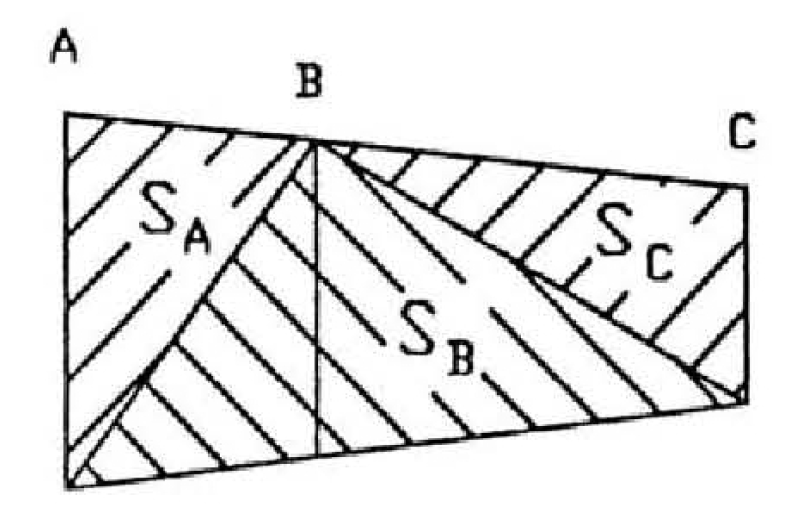
\includegraphics[height=3cm]{Immagini/influencearea}} 
%\caption{Influence area of the sections for finite wing.}
%\label{fig:influencearea}
%\end{figure}
%
%Then is possible to calculate the influence coefficients. 
%
%\begin{equation}
%K_i = \frac{2 S_i}{S}
%\end{equation}
%
%The mean parameters can be obtained from:
%
%\begin{equation}
%\overline{x} = x_1 K_1 + x_2 k_2 +x_3 k_3...
%\end{equation}
%
%In particular, for a wing defined by three airfoils, the end of linearity angle of attack is obtained from the following equation:
%
%\begin{equation}
%\alpha^* = \alpha^*_{1} K_1 + \alpha^*_{2} k_2 +\alpha^*_{3} k_3
%\end{equation}

\begin{flushright}
	{\smaller
		\textit{Once we accept our limits,\\  we go beyond them.}\\
		-- Albert Einstein}
\end{flushright}

\section{Induced Angle of Attack}
When a wing passes through the air, it creates a perturbation, which leads to a vertical component on the relative motion on the air over the wing. Consequently the air flow past the wing is inclined in regard of the initial free stream. Then, the wing behaves as thought the flow were coming from a different direction: the local flow direction.

\begin{figure}[H]
\centering
{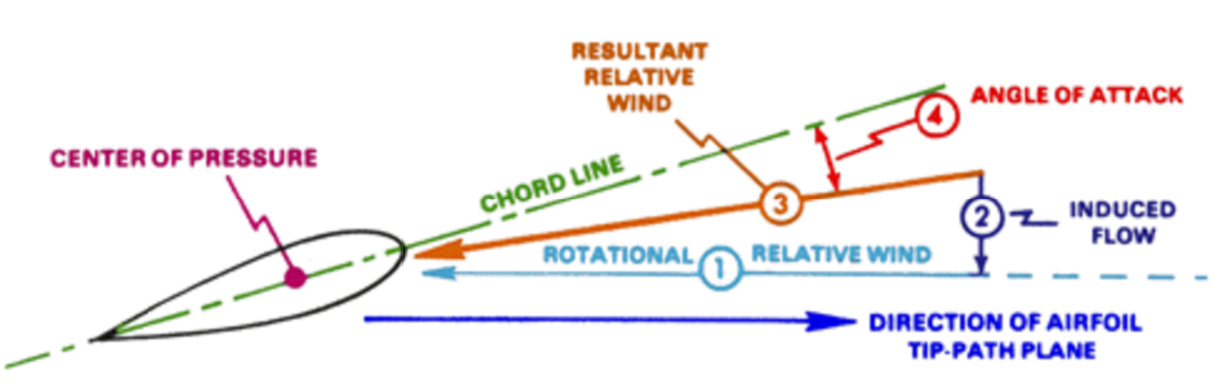
\includegraphics[height=3.9cm]{Immagini/induced}} 
\caption{Definitions of induced end effective angles of attack.}
\end{figure}

In practice, these perturbations are generated by the wingtip vortices, which create downwash and deflects the local airflow in the vicinity of the wing downward. This angle is the induced angle of attack $\alpha_i$. The airfoil section itself is then responding to an effective angle of attack equal to the geometric angle of attack minus the induced angle of attack: $\alpha_e=\alpha-\alpha_i$. In most cases, the absolute value of the angle of attack is decreased, and so as for the lift force. Then, in order to produce a given lift force, the AOA of the wing must be greater than the AOA that would be given by a theoretical study of the wing section (2D wing). Moreover, the resulting force exerted by the air on the wing, now perpendicular to the local flow direction, is tilted backwards by an angle equal to the induced angle of attack and then is no longer perpendicular to the free stream velocity. This important phenomenon is at the origin of the induced drag (i.e. the component of the resulting force parallel to the free stream velocity), and therefore for a given lift, a greater induced AOA implies a greater drag. One must bear in mind that because this is a 3-dimentional effect.\cite{induced}\\

In order to evaluate the effective angle of attack  for each spanwise station, it's possible to implement an iterative process in witch at a load distribution it's evaluated the related induced angles that generates a new load distribution.\\
The induced angle of attack is in eq. \ref{eq:alp},  where w is the vertical downwash component:

\begin{equation}
\alpha =\arctan\left( {\frac{w}{V}}\right )
\label{eq:alp}
\end{equation}

\begin{figure}[H]
\centering
{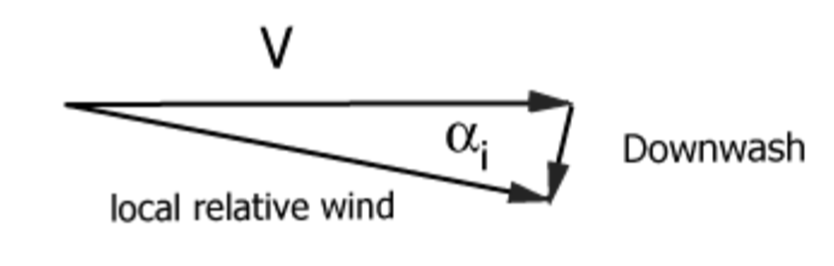
\includegraphics[height=1.6cm]{Immagini/atg}} 
\caption{Geometrical representation of induced angle of attack.}
\end{figure}

The lifting surfaces is considered as divided in several rectangular horse-shoe vortices along the span; one horseshoe vortex along the chord is used, that is, the midpoints of the vortices are placed only at points along the quarter-chord lines. An equal number of control points are located along the three-quarter-chord lines. The velocity from the total vortex system is equated to the component of free-stream velocity normal to the lifting surface chord at each control point.\\
The downwash velocity at any of the control points P, which results from the 2N horseshoe vortices is:

\begin{equation}
w = \frac{1}{4\pi} \sum_{n=1}^N \Gamma_N F'_{w,\nu_N}
\end{equation}

where $\Gamma$ is circulation strength, F is the downwash influence function, N are the vortex point and $\nu$ are the vortex points.\\
In JPAD this effect is calculated in the class \texttt{AlphaEffective} by the method \texttt{calculateAlphaEffective}. This method has as output an array of value that indicates the effective angls of attack semi-spanwise using the equations introduced before. In order to evaluate these angles you must have as input the operating conditions. 

\begin{lstlisting}[frame=rbl,caption={{\footnotesize Effective angle of attack Test Class}},label= [style=\bfseries]{Listing}]

// -----------------------------------------------------------------------
// Evaluate effective angle of attack
// -----------------------------------------------------------------------

System.out.println("\n \n-----------------------------------------------------");
System.out.println("STARTING EVALUATE EFFECTIVE ANGLE OF ATTACK ");
System.out.println("-----------------------------------------------------");

double[] alphaEffective;

AlphaEffective theAlphaCalculator = new AlphaEffective(
		theLSAnalysis, theWing, theOperatingConditions);
Amount<javax.measure.quantity.Angle> inputAngle = 
		Amount.valueOf(toRadians(8.), SI.RADIAN);

alphaEffective = theAlphaCalculator.calculateAlphaEffective(inputAngle);

System.out.println("\n \n-----------------------------------------------------");
System.out.println(" alpha --> " + inputAngle);
System.out.println(" alpha effective --> " + Arrays.toString(alphaEffective));

System.out.println("\n \n-----------------------------------------------------");
System.out.println("DONE");
System.out.println("-----------------------------------------------------");

\end{lstlisting}
